\section{Spark::Sp\-Tuple2$<$ Real $>$ Class Template Reference}
\label{classSpark_1_1SpTuple2}\index{Spark::SpTuple2@{Spark::SpTuple2}}
{\tt \#include $<$Sp\-Tuple.h$>$}

Inheritance diagram for Spark::Sp\-Tuple2$<$ Real $>$:\begin{figure}[H]
\begin{center}
\leavevmode
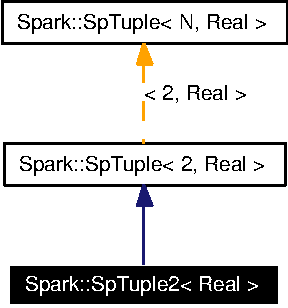
\includegraphics[width=86pt]{classSpark_1_1SpTuple2__inherit__graph}
\end{center}
\end{figure}
Collaboration diagram for Spark::Sp\-Tuple2$<$ Real $>$:\begin{figure}[H]
\begin{center}
\leavevmode
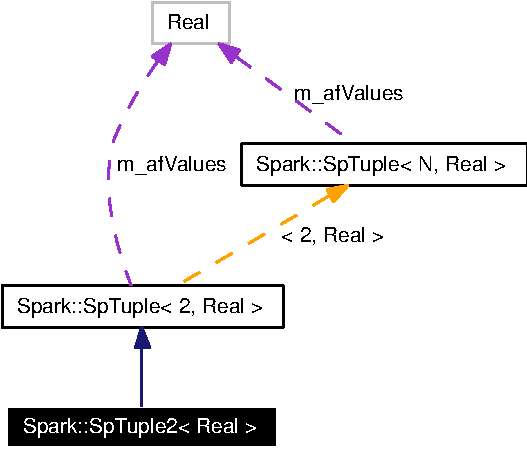
\includegraphics[width=144pt]{classSpark_1_1SpTuple2__coll__graph}
\end{center}
\end{figure}


\subsection{Detailed Description}
\subsubsection*{template$<$class Real$>$ class Spark::Sp\-Tuple2$<$ Real $>$}

2D tuple data class with support for vector mathematics 

Definition at line 107 of file Sp\-Tuple.h.\subsection*{Public Member Functions}
\begin{CompactItemize}
\item 
{\bf Sp\-Tuple2} (const {\bf Sp\-Tuple}$<$ 2, Real $>$ \&rk\-V)
\begin{CompactList}\small\item\em Construction. \item\end{CompactList}\item 
{\bf Sp\-Tuple2} (Real f\-X=0, Real f\-Y=0)
\item 
Real {\bf x} () const
\begin{CompactList}\small\item\em Position Coordinate Access:. \item\end{CompactList}\item 
Real \& {\bf x} ()
\item 
Real {\bf y} () const
\item 
Real \& {\bf y} ()
\item 
Real {\bf s} () const
\begin{CompactList}\small\item\em Texture Coordinate Access:. \item\end{CompactList}\item 
Real \& {\bf s} ()
\item 
Real {\bf t} () const
\item 
Real \& {\bf t} ()
\end{CompactItemize}


\subsection{Constructor \& Destructor Documentation}
\index{Spark::SpTuple2@{Spark::Sp\-Tuple2}!SpTuple2@{SpTuple2}}
\index{SpTuple2@{SpTuple2}!Spark::SpTuple2@{Spark::Sp\-Tuple2}}
\subsubsection{\setlength{\rightskip}{0pt plus 5cm}template$<$class Real$>$ {\bf Spark::Sp\-Tuple2}$<$ Real $>$::{\bf Sp\-Tuple2} (const {\bf Sp\-Tuple}$<$ 2, Real $>$ \& {\em rk\-V})\hspace{0.3cm}{\tt  [inline]}}\label{classSpark_1_1SpTuple2_a0}


Construction. 

Definition at line 113 of file Sp\-Tuple.h.\index{Spark::SpTuple2@{Spark::Sp\-Tuple2}!SpTuple2@{SpTuple2}}
\index{SpTuple2@{SpTuple2}!Spark::SpTuple2@{Spark::Sp\-Tuple2}}
\subsubsection{\setlength{\rightskip}{0pt plus 5cm}template$<$class Real$>$ {\bf Spark::Sp\-Tuple2}$<$ Real $>$::{\bf Sp\-Tuple2} (Real {\em f\-X} = {\tt 0}, Real {\em f\-Y} = {\tt 0})\hspace{0.3cm}{\tt  [inline]}}\label{classSpark_1_1SpTuple2_a1}


Definition at line 116 of file Sp\-Tuple.h.

References Spark::Sp\-Tuple2$<$ Real $>$::x(), and Spark::Sp\-Tuple2$<$ Real $>$::y().

\subsection{Member Function Documentation}
\index{Spark::SpTuple2@{Spark::Sp\-Tuple2}!s@{s}}
\index{s@{s}!Spark::SpTuple2@{Spark::Sp\-Tuple2}}
\subsubsection{\setlength{\rightskip}{0pt plus 5cm}template$<$class Real$>$ Real\& {\bf Spark::Sp\-Tuple2}$<$ Real $>$::s ()\hspace{0.3cm}{\tt  [inline]}}\label{classSpark_1_1SpTuple2_a7}


Definition at line 131 of file Sp\-Tuple.h.\index{Spark::SpTuple2@{Spark::Sp\-Tuple2}!s@{s}}
\index{s@{s}!Spark::SpTuple2@{Spark::Sp\-Tuple2}}
\subsubsection{\setlength{\rightskip}{0pt plus 5cm}template$<$class Real$>$ Real {\bf Spark::Sp\-Tuple2}$<$ Real $>$::s () const\hspace{0.3cm}{\tt  [inline]}}\label{classSpark_1_1SpTuple2_a6}


Texture Coordinate Access:. 

Definition at line 130 of file Sp\-Tuple.h.\index{Spark::SpTuple2@{Spark::Sp\-Tuple2}!t@{t}}
\index{t@{t}!Spark::SpTuple2@{Spark::Sp\-Tuple2}}
\subsubsection{\setlength{\rightskip}{0pt plus 5cm}template$<$class Real$>$ Real\& {\bf Spark::Sp\-Tuple2}$<$ Real $>$::t ()\hspace{0.3cm}{\tt  [inline]}}\label{classSpark_1_1SpTuple2_a9}


Definition at line 133 of file Sp\-Tuple.h.\index{Spark::SpTuple2@{Spark::Sp\-Tuple2}!t@{t}}
\index{t@{t}!Spark::SpTuple2@{Spark::Sp\-Tuple2}}
\subsubsection{\setlength{\rightskip}{0pt plus 5cm}template$<$class Real$>$ Real {\bf Spark::Sp\-Tuple2}$<$ Real $>$::t () const\hspace{0.3cm}{\tt  [inline]}}\label{classSpark_1_1SpTuple2_a8}


Definition at line 132 of file Sp\-Tuple.h.\index{Spark::SpTuple2@{Spark::Sp\-Tuple2}!x@{x}}
\index{x@{x}!Spark::SpTuple2@{Spark::Sp\-Tuple2}}
\subsubsection{\setlength{\rightskip}{0pt plus 5cm}template$<$class Real$>$ Real\& {\bf Spark::Sp\-Tuple2}$<$ Real $>$::x ()\hspace{0.3cm}{\tt  [inline]}}\label{classSpark_1_1SpTuple2_a3}


Definition at line 123 of file Sp\-Tuple.h.\index{Spark::SpTuple2@{Spark::Sp\-Tuple2}!x@{x}}
\index{x@{x}!Spark::SpTuple2@{Spark::Sp\-Tuple2}}
\subsubsection{\setlength{\rightskip}{0pt plus 5cm}template$<$class Real$>$ Real {\bf Spark::Sp\-Tuple2}$<$ Real $>$::x () const\hspace{0.3cm}{\tt  [inline]}}\label{classSpark_1_1SpTuple2_a2}


Position Coordinate Access:. 

Definition at line 122 of file Sp\-Tuple.h.

Referenced by Spark::Sp\-Tuple2$<$ Real $>$::Sp\-Tuple2().\index{Spark::SpTuple2@{Spark::Sp\-Tuple2}!y@{y}}
\index{y@{y}!Spark::SpTuple2@{Spark::Sp\-Tuple2}}
\subsubsection{\setlength{\rightskip}{0pt plus 5cm}template$<$class Real$>$ Real\& {\bf Spark::Sp\-Tuple2}$<$ Real $>$::y ()\hspace{0.3cm}{\tt  [inline]}}\label{classSpark_1_1SpTuple2_a5}


Definition at line 125 of file Sp\-Tuple.h.\index{Spark::SpTuple2@{Spark::Sp\-Tuple2}!y@{y}}
\index{y@{y}!Spark::SpTuple2@{Spark::Sp\-Tuple2}}
\subsubsection{\setlength{\rightskip}{0pt plus 5cm}template$<$class Real$>$ Real {\bf Spark::Sp\-Tuple2}$<$ Real $>$::y () const\hspace{0.3cm}{\tt  [inline]}}\label{classSpark_1_1SpTuple2_a4}


Definition at line 124 of file Sp\-Tuple.h.

Referenced by Spark::Sp\-Tuple2$<$ Real $>$::Sp\-Tuple2().

The documentation for this class was generated from the following file:\begin{CompactItemize}
\item 
{\bf Sp\-Tuple.h}\end{CompactItemize}
